\newcommand{\doctitle}{Construct and Destroy \\ Test Document}
\newcommand{\doctitleshort}{C\&D Test Document}

\newcommand{\docauthor} {
    \renewcommand{\arraystretch}{0.5}
    \begin{tabular}{l l}
        \textbf{Students:} & ~ \\
        Mark van der Woude     & {\mdseries(S1081655)} \\
        Stephan Schrijver     & {\mdseries(S1078783)} \\
        Jeroen Vinke     & {\mdseries(S1078666)} \\
        Sander Bouwman   & {\mdseries(S1080528)} \\
        Robin T. Koning  & {\mdseries(S1078710)} \\
    \end{tabular}
}

\newcommand{\doctitlepage} {
    \thispagestyle{empty}
    \parbox[t]{1.0\linewidth}{
        \fontsize{40pt}{60pt}\selectfont
        \vspace*{1.5cm}
        \doctitle{}
        \vspace*{1.5cm}
    }
    \vfill
    {
        \centering
        \large
        \hfill \today
        \hfill \docauthor{}
    }
    \normalcolor{}

    \newpage
}

\providecommand{\doctitle}{Title}
\providecommand{\docauthor}{Author}
\providecommand{\doctype}{scrartcl}
\providecommand{\doctitlepage}{TitlePage}

\documentclass[12pt,a4paper,titlepage,parskip=full]{\doctype}

\PassOptionsToPackage{table,xcdraw}{xcolor}

\usepackage[english]{babel}
\usepackage{caption}
\usepackage{float}
\usepackage{blindtext}
\usepackage{hyperref}
\usepackage{graphicx}
\usepackage{listings}
\usepackage{tikz}
\usetikzlibrary{decorations.pathreplacing}
\usepackage{pdfpages}
\usepackage{apacite}
\usepackage{tabularx}
\bibliographystyle{apacite}

% set Listing settings -------------------------------------
\usepackage{listings}
\usepackage{color}

% Input and output encoding ---------------------------------------------------
\usepackage{iftex}
\ifPDFTeX
   \usepackage[utf8]{inputenc}
   \usepackage[T1]{fontenc}
   \usepackage{lmodern}
\else
   \ifXeTeX
     \usepackage{xltxtra}
   \else
     \usepackage{luatextra}
   \fi
   \defaultfontfeatures{Ligatures=TeX}
\fi

% Math
\usepackage{amsmath}
\usepackage{amsfonts}
\usepackage{amsthm}
\usepackage{amssymb}
\usepackage{mathtools}
\usepackage{bm}
\newcommand{\uvec}[1]{\boldsymbol{\hat{\textbf{#1}}}}

\DeclarePairedDelimiter{\ceil}{\lceil}{\rceil}
\DeclarePairedDelimiter{\floor}{\lfloor}{\rfloor}
\DeclarePairedDelimiter{\bag}{\langle}{\rangle}
\DeclarePairedDelimiter{\set}{\{}{\}}

% Misc
\usepackage{marginnote}
\usepackage[shortlabels]{enumitem}

% Display
\usepackage{lastpage}
\usepackage{fancyhdr}
\setlength{\headheight}{24pt}
\usepackage{eurosym}
\pagestyle{fancy}

\usepackage[nameinlink]{cleveref}

\title{\doctitle}
\author{\docauthor}
\date{\today}

\lhead{\doctitleshort}
\rhead{\today}
\cfoot{\thepage\ /~\pageref{LastPage}}
%\lfoot{\docauthor}

\numberwithin{equation}{section}
\numberwithin{figure}{section}
\numberwithin{table}{section}

\usepackage{changepage}

%Other settings

% Code listing settings
\definecolor{back-color}{rgb}{1,1,1}
\definecolor{keywords}{rgb}{0.654,0.113,0.364}
\definecolor{comments}{rgb}{0.588,0.596,0.588}
\definecolor{strings}{rgb}{0.094,0.211,0.568}

\lstdefinestyle{c++} {
    % Basic settings
    language=[ISO]C++,
    frame=tb,
    tabsize=4,
    showspaces=false,
    showtabs=false,
    showstringspaces=false,
    captionpos=b,
    breaklines=true,
    breakatwhitespace=true,
    numbers=left,
    basicstyle=\scriptsize\ttfamily,
    % Color settings
    backgroundcolor=\color{back-color},
    keywordstyle=\color{keywords},
    commentstyle=\color{comments},
    stringstyle=\color{strings}
}
\lstset{style=c++}

\begin{document}
\doctitlepage{}

\tableofcontents
\thispagestyle{empty}
\newpage

\clearpage
\setcounter{page}{1}
\addtocontents{toc}{\protect\thispagestyle{empty}}
\newpage

% Abstract, the intro to our document
\begin{abstract}
\blindtext
\end{abstract}

\newpage

%----------------------------------
\section{Functionalities}
\subsection{Placing buildings}

\begin{tabularx}{\textwidth}{|X|X|}
\hline
\rowcolor{lightgray}\textcolor{white}{\textbf{Test scenario}} &
\textcolor{white}{\textbf{Desired result}}       
\\\hline
Positioning a building & A building can be positioned and appears at the center of the cursor when a player clicks on a building in the building panel
\\\hline
\rowcolor{lightgray}\textcolor{white}{\textbf{Comments/suggestions}} & 
\textcolor{white}{\textbf{Passed}}
\\\hline
 & \cellcolor{green}                       
\\\hline
\rowcolor{lightgray}\textcolor{white}{\textbf{Tester}} & 
\textcolor{white}{\textbf{Date}}               
\\\hline
Mark van der Woude & May 8, 2017                               		 
\\\hline
\end{tabularx}

\begin{tabularx}{\textwidth}{|X|X|}
\hline
\rowcolor{lightgray}\textcolor{white}{\textbf{Test scenario}} &
\textcolor{white}{\textbf{Desired result}}       
\\\hline
Placing a building &
When a player clicks somewhere in the world while positioning a building, the building should be added to the world       
\\\hline
\rowcolor{lightgray}\textcolor{white}{\textbf{Comments/suggestions}} & 
\textcolor{white}{\textbf{Passed}}
\\\hline
 & \cellcolor{green}                       
\\\hline
\rowcolor{lightgray}\textcolor{white}{\textbf{Tester}} & 
\textcolor{white}{\textbf{Date}}               
\\\hline
Mark van der Woude & May 8, 2017                               		 
\\\hline
\end{tabularx}

\begin{tabularx}{\textwidth}{|X|X|}
\hline
\rowcolor{lightgray}\textcolor{white}{\textbf{Test scenario}} &
\textcolor{white}{\textbf{Desired result}}       
\\\hline
Trying to place a building on top of another static entity &
A building cannot be positioned on top of an existing building or resource (tree, campfire et cetera), and should give the player feedback when it tries to position on top of it
\\\hline
\rowcolor{lightgray}\textcolor{white}{\textbf{Comments/suggestions}} & 
\textcolor{white}{\textbf{Passed}}
\\\hline
Building in positioning state gets a red border while hovering over another static entity & \cellcolor{green}                       
\\\hline
\rowcolor{lightgray}\textcolor{white}{\textbf{Tester}} & 
\textcolor{white}{\textbf{Date}}               
\\\hline
Mark van der Woude & May 8, 2017                               		 
\\\hline
\end{tabularx}
\section{Creating units}
In this chapter we will explain how creating units is implemented in the game. We will go through some of the code and show the design patterns we used.

\subsection{Entity Panel} \label{sec:EntityPanel}
A unit can be created in a building, in a castle for example. When the player selects a castle the building panel is replaced by a different panel which shows all units that can be spawned from the selected building. This can be seen in \cref{fig:entity-panel}, where the entity panel is the panel at the bottom of the screen. 

A player can order many entities, but they won't be spawned right away. Instead, they are queued. The number of entities in the build queue are displayed in a badge. Only one entity can be spawned at a given time. The color of the badge indicates whether an entity is being built and how close it is to actually spawning. 

All variations of the badge can be seen in \cref{fig:unit-panel-order-queue}. If there aren't any entities in the queue, then the badge is grey. If there are entities in the queue, but it isn't currently being built, then the badge is grey as well. When an entity is building, the badge has a red background at first which slowly changes to green over time, and is solid green just before the entity gets spawned.

The cost of spawning an entity can be seen below each entity itself in the panel. The cost will turn red if the player does not have sufficient resources to train the entity. 

If the player wants additional information about something the available entities in the panel the player can hover over the units image. This will trigger a description in the topleft corner giving a short explanation of what the entity does. E.g. for a Knight the description will say something like: "This unit will fight for the safety of you village" and for a lumberjack it will say: "This unit will gather wood."

In \cref{fig:unit-panel} all unit panels are highlighted. For each unit that can be spawned from the selected building, a unit panel is added to the entity panel at the bottom of the screen. A unit panel, as displayed in \cref{fig:unit-panel-class-diagram}, contains the EntityType that belongs to a unit panel which it uses to render the sprite that belongs to the EntityType.

In order to capture click events, and trigger the unit spawning process, a MouseHandlerEntityPanel is used. When the player clicks on an entity, the mouse handler takes care of spawning the unit and subtracing the resource cost. The entity will only be ordered if the player has enough resources to pay for the unit, as shown below.

Another way to spawn a unit is to press the shortcut key. This shortcut key is shown in the top left badge of the unit panel, as you can see in  \cref{fig:entity-shortcuts}.

\begin{lstlisting}
 if (p->resources->check_if_sufficient_resources(spawnable_entity->get_cost())) {
    // tell the building to spawn the selected entity type
    building->order_unit(spawnable_entity->get_entity_type());
    
    p->resources->subtract_resources(spawnable_entity->get_cost());
}
\end{lstlisting}

\subsection{Ordering units}
When a user orders a unit from a building we will look at the order time of the castle which represents the time the castle needs to create the unit. This time can be seen as time that is needed to train the unit and make it ready to participate in your world to give it a more realistic feeling than spawning the unit immediately on the screen. 

When the player orders a unit. The following method is called:

\begin{lstlisting}
void CastleEntity::order_unit(MovingEntityType moving_entity_type) {
    this->orders.push_back(moving_entity_type);
}
\end{lstlisting}

We add the type of the unit to a vector called orders. In which the orders placed by the player on that building are saved. The order is pushed to the back of the vector so that the array somewhat resembles a queue. A enum member of the enum MovingEntityType is used to determine what kind of unit needs to be created. After the completion of this method a unit is successfully ordered and waits for time to pass to be created.

\subsection{Handling the orders}
To handle orders placed in the building we use the update method. The update method is called every game-update so it is perfect to calculate time and decide if anything needs to be done with the orders. Below you can see the code of the update method:

%-- Do not worry about the code listings being half on two different pages. This will be fixed when Jeroen is done. 

\begin{lstlisting}
void CastleEntity::update(float d) {
    if(!this->orders.empty()){
        delta_time += d;
        if(delta_time >= order_time){


            this->order_unit_from_factory(_player, spawn, orders.front());

            //remove first from orders.
            orders.erase(orders.begin());
 
            //reset order time.
            delta_time = 0;
        }
    };
}
\end{lstlisting}

First we check if order is not empty. If that is the case, we update the delta\_time. This is so we know the time that has passed since the an order was placed. Then we check if the order\_time, the time it takes to create a unit, has been surpassed by the time that has passed since the order was placed. If that is the case we handle off the order of the unit by calling the method order\_unit\_from\_factory which we will explain below. After ordering from the factory, we take out the order from the orders vector since the order has been handled. And we also reset the delta\_time to zero so we can handle the next order after the same order\_time.

\subsection{MovingEntity Factory}
The order\_unit\_from\_factory method calls the MovingEntityManager's method add\_unit. As parameters it provides:

\begin{itemize}  
\item A Player*, the player for which the unit has to be created.
\item A vec2 Position, the X and Y coordinates where the unit should be spawned.
\item A MovingEntityType, type of the unit(FE: Lumberjack, Miner, Knight and more...)
\end{itemize}
The MovingEntityManager handles any interaction with the factory. And uses the parameters to call the factory and create the unit. We have implemented the structure of this code like a factory pattern as can be seen in the following class diagram below. The class diagram found at \cref{fig:movingentityfactory} focusses on the factory and the classes that use and so only the really important classes are completely shown with all it's methods and attributes.  

After the MovingEntityManager has completed an order from the factory the unit will spawn in the given location. This process will repeat until all orders have been handled.





\subsection{Selecting units}

\begin{tabularx}{\textwidth}{|X|X|}
\hline
\rowcolor{lightgray}\textcolor{white}{\textbf{Test scenario}} &
\textcolor{white}{\textbf{Desired result}}       
\\\hline
Selecting a unit by clicking on it. & The unit that was clicked on gets selected.       
\\\hline
\rowcolor{lightgray}\textcolor{white}{\textbf{Comments/suggestions}} & 
\textcolor{white}{\textbf{Passed}}
\\\hline
Some precision is needed when clicking on the unit. & \cellcolor{green}                      
\\\hline
\rowcolor{lightgray}\textcolor{white}{\textbf{Tester}} & 
\textcolor{white}{\textbf{Date}}               
\\\hline
Mark van der Woude & May 8, 2017                               		 
\\\hline
\end{tabularx}

\begin{tabularx}{\textwidth}{|X|X|}
\hline
\rowcolor{lightgray}\textcolor{white}{\textbf{Test scenario}} &
\textcolor{white}{\textbf{Desired result}}       
\\\hline
Dragging the mouse of the screen while holding down the left button. & A selection rectangle is drawn from the point the user pressed the left button to the position the mouse is currently at.       
\\\hline
\rowcolor{lightgray}\textcolor{white}{\textbf{Comments/suggestions}} & 
\textcolor{white}{\textbf{Passed}}
\\\hline
Some precision is needed when clicking on the unit. & \cellcolor{green}                      
\\\hline
\rowcolor{lightgray}\textcolor{white}{\textbf{Tester}} & 
\textcolor{white}{\textbf{Date}}               
\\\hline
Mark van der Woude & May 8, 2017                               		 
\\\hline
\end{tabularx}

\begin{tabularx}{\textwidth}{|X|X|}
\hline
\rowcolor{lightgray}\textcolor{white}{\textbf{Test scenario}} &
\textcolor{white}{\textbf{Desired result}}       
\\\hline
Dragging a selection rectangle around multiple units at the same time. & All units in the rectangle get selected.   
\\\hline
\rowcolor{lightgray}\textcolor{white}{\textbf{Comments/suggestions}} & 
\textcolor{white}{\textbf{Passed}}
\\\hline
Some precision is needed when clicking on the unit. & \cellcolor{green}                      
\\\hline
\rowcolor{lightgray}\textcolor{white}{\textbf{Tester}} & 
\textcolor{white}{\textbf{Date}}               
\\\hline
Mark van der Woude & May 8, 2017                               		 
\\\hline
\end{tabularx}


\begin{tabularx}{\textwidth}{|X|X|}
\hline
\rowcolor{lightgray}\textcolor{white}{\textbf{Test scenario}} &
\textcolor{white}{\textbf{Desired result}}       
\\\hline
Selecting units. & Units should be selected and a red line should be drawn around them.  
\\\hline
\rowcolor{lightgray}\textcolor{white}{\textbf{Comments/suggestions}} & 
\textcolor{white}{\textbf{Passed}}
\\\hline
Some precision is needed when clicking on the unit. & \cellcolor{green}                      
\\\hline
\rowcolor{lightgray}\textcolor{white}{\textbf{Tester}} &
\textcolor{white}{\textbf{Date}}               
\\\hline
Mark van der Woude & May 8, 2017                               		 
\\\hline
\end{tabularx}


\begin{tabularx}{\textwidth}{|X|X|}
\hline
\rowcolor{lightgray}\textcolor{white}{\textbf{Test scenario}} &
\textcolor{white}{\textbf{Desired result}}       
\\\hline
Left click somewhere on an empty spot in the world while having units selected. & Units should be deselected.  
\\\hline
\rowcolor{lightgray}\textcolor{white}{\textbf{Comments/suggestions}} & 
\textcolor{white}{\textbf{Passed}}
\\\hline
Some precision is needed when clicking on the unit. & \cellcolor{green}                      
\\\hline
\rowcolor{lightgray}\textcolor{white}{\textbf{Tester}} & 
\textcolor{white}{\textbf{Date}}               
\\\hline
Mark van der Woude & May 8, 2017                               		 
\\\hline
\end{tabularx}


\begin{tabularx}{\textwidth}{|X|X|}
\hline
\rowcolor{lightgray}\textcolor{white}{\textbf{Test scenario}} &
\textcolor{white}{\textbf{Desired result}}       
\\\hline
Left click on a unit while having multiple units selected. & All units should be deselected except for the unit that clicked on.  
\\\hline
\rowcolor{lightgray}\textcolor{white}{\textbf{Comments/suggestions}} & 
\textcolor{white}{\textbf{Passed}}
\\\hline
Some precision is needed when clicking on the unit. & \cellcolor{green}                      
\\\hline
\rowcolor{lightgray}\textcolor{white}{\textbf{Tester}} & 
\textcolor{white}{\textbf{Date}}               
\\\hline
Mark van der Woude & May 8, 2017                               		 
\\\hline
\end{tabularx}
\subsection{Controlling workers}

\begin{tabularx}{\textwidth}{|X|X|}
\hline
\rowcolor{lightgray}\textcolor{white}{\textbf{Test scenario}} &
\textcolor{white}{\textbf{Desired result}}       
\\\hline
Let one worker move to a position & After a player selects a worker and clicks on the ground, the worker should walk to that position        
\\\hline
\rowcolor{lightgray}\textcolor{white}{\textbf{Comments/suggestions}} & 
\textcolor{white}{\textbf{Passed}}
\\\hline
 & \cellcolor{green}                       
\\\hline
\rowcolor{lightgray}\textcolor{white}{\textbf{Tester}} & \cellcolor{lightgray}\textcolor{white}{\textbf{Date}}               
\\\hline
Mark van der Woude & May 8, 2017                               		 
\\\hline
\end{tabularx}

\begin{tabularx}{\textwidth}{|X|X|}
\hline
\rowcolor{lightgray}\textcolor{white}{\textbf{Test scenario}} &
\textcolor{white}{\textbf{Desired result}}       
\\\hline
Let multiple workers move to a position & After a player selects a worker and clicks on the ground, the worker should walk to that position        
\\\hline
\rowcolor{lightgray}\textcolor{white}{\textbf{Comments/suggestions}} & 
\textcolor{white}{\textbf{Passed}}
\\\hline
 & \cellcolor{green}                       
\\\hline
\rowcolor{lightgray}\textcolor{white}{\textbf{Tester}} & \cellcolor{lightgray}\textcolor{white}{\textbf{Date}}               
\\\hline
Mark van der Woude & May 8, 2017                               		 
\\\hline
\end{tabularx}
\subsection{Combat}

\begin{tabularx}{\textwidth}{|X|X|}
\hline
\rowcolor{lightgray}\textcolor{white}{\textbf{Test scenario}} &
\textcolor{white}{\textbf{Desired result}}       
\\\hline
Attack a moving entity. &
If the moving entity has moved too much a new path should be planned.         
\\\hline
\rowcolor{lightgray}\textcolor{white}{\textbf{Comments/suggestions}} & 
\textcolor{white}{\textbf{Passed}}
\\\hline
 & \cellcolor{green}                       
\\\hline
\rowcolor{lightgray}\textcolor{white}{\textbf{Tester}} & 
\textcolor{white}{\textbf{Date}}               
\\\hline
Sander Bouwman & May 24, 2017                               		 
\\\hline
\end{tabularx}

\begin{tabularx}{\textwidth}{|X|X|}
\hline
\rowcolor{lightgray}\textcolor{white}{\textbf{Test scenario}} &
\textcolor{white}{\textbf{Desired result}}       
\\\hline
An entity is killed while other entities are hunting that entity, meaning not yet reached their target. &
The entities that are hunting that target should stop and find another target.       
\\\hline
\rowcolor{lightgray}\textcolor{white}{\textbf{Comments/suggestions}} & 
\textcolor{white}{\textbf{Passed}}
\\\hline
 & \cellcolor{green}                       
\\\hline
\rowcolor{lightgray}\textcolor{white}{\textbf{Tester}} & 
\textcolor{white}{\textbf{Date}}               
\\\hline
Sander Bouwman & May 24, 2017                               		 
\\\hline
\end{tabularx}

\begin{tabularx}{\textwidth}{|X|X|}
\hline
\rowcolor{lightgray}\textcolor{white}{\textbf{Test scenario}} &
\textcolor{white}{\textbf{Desired result}}       
\\\hline
Attacking an entity. &
Entity is taking damage which is shown with the health bar above the entity. 
\\\hline
\rowcolor{lightgray}\textcolor{white}{\textbf{Comments/suggestions}} & 
\textcolor{white}{\textbf{Passed}}
\\\hline
 & \cellcolor{green}                       
\\\hline
\rowcolor{lightgray}\textcolor{white}{\textbf{Tester}} & 
\textcolor{white}{\textbf{Date}}               
\\\hline
Sander Bouwman & May 24, 2017                               		 
\\\hline
\end{tabularx}

\begin{tabularx}{\textwidth}{|X|X|}
\hline
\rowcolor{lightgray}\textcolor{white}{\textbf{Test scenario}} &
\textcolor{white}{\textbf{Desired result}}       
\\\hline
Spawn an enemy entity.&
An entity of the player with the combat goal should attack the enemy entity.
\\\hline
\rowcolor{lightgray}\textcolor{white}{\textbf{Comments/suggestions}} & 
\textcolor{white}{\textbf{Passed}}
\\\hline
 & \cellcolor{green}                       
\\\hline
\rowcolor{lightgray}\textcolor{white}{\textbf{Tester}} &
\textcolor{white}{\textbf{Date}}               
\\\hline
Sander Bouwman& May 24, 2017                               		 
\\\hline
\end{tabularx}

\begin{tabularx}{\textwidth}{|X|X|}
\hline
\rowcolor{lightgray}\textcolor{white}{\textbf{Test scenario}} &
\textcolor{white}{\textbf{Desired result}}       
\\\hline
Spawn a wave of enemy entities.&
The entities that have spawned should start attacking entities of the player.        
\\\hline
\rowcolor{lightgray}\textcolor{white}{\textbf{Comments/suggestions}} & 
\textcolor{white}{\textbf{Passed}}
\\\hline
 & \cellcolor{green}                       
\\\hline
\rowcolor{lightgray}\textcolor{white}{\textbf{Tester}} & 
\textcolor{white}{\textbf{Date}}               
\\\hline
Sander Bouwman & May 24, 2017                               		 
\\\hline
\end{tabularx}

\begin{tabularx}{\textwidth}{|X|X|}
\hline
\rowcolor{lightgray}\textcolor{white}{\textbf{Test scenario}} &
\textcolor{white}{\textbf{Desired result}}       
\\\hline
Attacking a worker. &
If the worker survives the fight it should continue doing his job, e.g. a lumberjack should continue gathering wood.        
\\\hline
\rowcolor{lightgray}\textcolor{white}{\textbf{Comments/suggestions}} & 
\textcolor{white}{\textbf{Passed}}
\\\hline
 & \cellcolor{green}                       
\\\hline
\rowcolor{lightgray}\textcolor{white}{\textbf{Tester}} & 
\textcolor{white}{\textbf{Date}}               
\\\hline
Sander Bouwman & May 24, 2017                               		 
\\\hline
\end{tabularx}

\begin{tabularx}{\textwidth}{|X|X|}
\hline
\rowcolor{lightgray}\textcolor{white}{\textbf{Test scenario}} &
\textcolor{white}{\textbf{Desired result}}       
\\\hline
Attacking an entity. &
When an entity is attacked it should start fighting back.
\\\hline
\rowcolor{lightgray}\textcolor{white}{\textbf{Comments/suggestions}} & 
\textcolor{white}{\textbf{Passed}}
\\\hline
 & \cellcolor{green}                       
\\\hline
\rowcolor{lightgray}\textcolor{white}{\textbf{Tester}} & 
\textcolor{white}{\textbf{Date}}               
\\\hline
Sander Bouwman & May 24, 2017                               		 
\\\hline
\end{tabularx}

\begin{tabularx}{\textwidth}{|X|X|}
\hline
\rowcolor{lightgray}\textcolor{white}{\textbf{Test scenario}} &
\textcolor{white}{\textbf{Desired result}}       
\\\hline
Killing an entity. &
If an entity with the combat goal survives it should start looking for other entities to kill.      
\\\hline
\rowcolor{lightgray}\textcolor{white}{\textbf{Comments/suggestions}} & 
\textcolor{white}{\textbf{Passed}}
\\\hline
 & \cellcolor{green}                       
\\\hline
\rowcolor{lightgray}\textcolor{white}{\textbf{Tester}} & 
\textcolor{white}{\textbf{Date}}               
\\\hline
Sander Bouwman & May 24, 2017                               		 
\\\hline
\end{tabularx}

\begin{tabularx}{\textwidth}{|X|X|}
\hline
\rowcolor{lightgray}\textcolor{white}{\textbf{Test scenario}} &
\textcolor{white}{\textbf{Desired result}}       
\\\hline
Killing an entity. &
If an entity dies it should be removed from the map/game.
\\\hline
\rowcolor{lightgray}\textcolor{white}{\textbf{Comments/suggestions}} & 
\textcolor{white}{\textbf{Passed}}
\\\hline
 & \cellcolor{green}                       
\\\hline
\rowcolor{lightgray}\textcolor{white}{\textbf{Tester}} & 
\textcolor{white}{\textbf{Date}}               
\\\hline
Sander Bouwman & May 24, 2017                               		 
\\\hline
\end{tabularx}

\begin{tabularx}{\textwidth}{|X|X|}
\hline
\rowcolor{lightgray}\textcolor{white}{\textbf{Test scenario}} &
\textcolor{white}{\textbf{Desired result}}       
\\\hline
All entities of the player are dead. &
The AI should start attacking buildings.       
\\\hline
\rowcolor{lightgray}\textcolor{white}{\textbf{Comments/suggestions}} & 
\textcolor{white}{\textbf{Passed}}
\\\hline
 & \cellcolor{green}                       
\\\hline
\rowcolor{lightgray}\textcolor{white}{\textbf{Tester}} & 
\textcolor{white}{\textbf{Date}}               
\\\hline
Sander Bouwman & May 24, 2017                               		 
\\\hline
\end{tabularx}

\begin{tabularx}{\textwidth}{|X|X|}
\hline
\rowcolor{lightgray}\textcolor{white}{\textbf{Test scenario}} &
\textcolor{white}{\textbf{Desired result}}       
\\\hline
All entities of the AI are dead. &
The entities of the player should start wandering around.
\\\hline
\rowcolor{lightgray}\textcolor{white}{\textbf{Comments/suggestions}} & 
\textcolor{white}{\textbf{Passed}}
\\\hline
 & \cellcolor{green}                       
\\\hline
\rowcolor{lightgray}\textcolor{white}{\textbf{Tester}} & 
\textcolor{white}{\textbf{Date}}               
\\\hline
Sander Bouwman & May 24, 2017                               		 
\\\hline
\end{tabularx}

\subsection{Work}

\begin{tabularx}{\textwidth}{|X|X|}
\hline
\rowcolor{lightgray}\textcolor{white}{\textbf{Test scenario}} &
\textcolor{white}{\textbf{Desired result}}       
\\\hline
Gathering resources.&
Resources should be extraced from the resource entity, e.g. from the goldmine, and should be added to the gathering entity.
\\\hline
\rowcolor{lightgray}\textcolor{white}{\textbf{Comments/suggestions}} & 
\textcolor{white}{\textbf{Passed}}
\\\hline
 & \cellcolor{green}                       
\\\hline
\rowcolor{lightgray}\textcolor{white}{\textbf{Tester}} & 
\textcolor{white}{\textbf{Date}}               
\\\hline
Sander Bouwman & May 7, 2017                               		 
\\\hline
\end{tabularx}

\begin{tabularx}{\textwidth}{|X|X|}
\hline
\rowcolor{lightgray}\textcolor{white}{\textbf{Test scenario}} &
\textcolor{white}{\textbf{Desired result}}       
\\\hline
Dropping resources. &
Resources should be removed from the gather entity and added to the player.
\\\hline
\rowcolor{lightgray}\textcolor{white}{\textbf{Comments/suggestions}} & 
\textcolor{white}{\textbf{Passed}}
\\\hline
 & \cellcolor{green}                       
\\\hline
\rowcolor{lightgray}\textcolor{white}{\textbf{Tester}} & 
\textcolor{white}{\textbf{Date}}               
\\\hline
Sander Bouwman & May 7, 2017                               		 
\\\hline
\end{tabularx}

\begin{tabularx}{\textwidth}{|X|X|}
\hline
\rowcolor{lightgray}\textcolor{white}{\textbf{Test scenario}} &
\textcolor{white}{\textbf{Desired result}}       
\\\hline
A resource entity is depleted. &
Resource entities should replenish resources slowly over time.\\\hline
\rowcolor{lightgray}\textcolor{white}{\textbf{Comments/suggestions}} & 
\textcolor{white}{\textbf{Passed}}
\\\hline
 & \cellcolor{green}                       
\\\hline
\rowcolor{lightgray}\textcolor{white}{\textbf{Tester}} & 
\textcolor{white}{\textbf{Date}}               
\\\hline
Sander Bouwman & May 7, 2017                               		 
\\\hline
\end{tabularx}

\begin{tabularx}{\textwidth}{|X|X|}
\hline
\rowcolor{lightgray}\textcolor{white}{\textbf{Test scenario}} &
\textcolor{white}{\textbf{Desired result}}       
\\\hline
All resources of a certain type, e.g. trees, are depleted. &
The corresponding workers can't continue gathering, in this case lumberjacks can't gather wood anymore.
\\\hline
\rowcolor{lightgray}\textcolor{white}{\textbf{Comments/suggestions}} & 
\textcolor{white}{\textbf{Passed}}
\\\hline
 & \cellcolor{green}                       
\\\hline
\rowcolor{lightgray}\textcolor{white}{\textbf{Tester}} & 
\textcolor{white}{\textbf{Date}}               
\\\hline
Sander Bouwman & May 7, 2017                               		 
\\\hline
\end{tabularx}

\begin{tabularx}{\textwidth}{|X|X|}
\hline
\rowcolor{lightgray}\textcolor{white}{\textbf{Test scenario}} &
\textcolor{white}{\textbf{Desired result}}       
\\\hline
There is no warehouse on the map. &
The worker will gather his resources but after that he won't do anything until a warehouse is placed.
\\\hline
\rowcolor{lightgray}\textcolor{white}{\textbf{Comments/suggestions}} & 
\textcolor{white}{\textbf{Passed}}
\\\hline
 & \cellcolor{green}                       
\\\hline
\rowcolor{lightgray}\textcolor{white}{\textbf{Tester}} & 
\textcolor{white}{\textbf{Date}}               
\\\hline
Sander Bouwman & May 7, 2017                               		 
\\\hline
\end{tabularx}

\begin{tabularx}{\textwidth}{|X|X|}
\hline
\rowcolor{lightgray}\textcolor{white}{\textbf{Test scenario}} &
\textcolor{white}{\textbf{Desired result}}       
\\\hline
Gathering resources.&
Lumberjacks should gather wood, goldminers should mine gold, etc..
\\\hline
\rowcolor{lightgray}\textcolor{white}{\textbf{Comments/suggestions}} & 
\textcolor{white}{\textbf{Passed}}
\\\hline
 & \cellcolor{green}                       
\\\hline
\rowcolor{lightgray}\textcolor{white}{\textbf{Tester}} & 
\textcolor{white}{\textbf{Date}}               
\\\hline
Sander Bouwman & May 7, 2017                               		 
\\\hline
\end{tabularx}

\subsection{Resource Panel}

\begin{tabularx}{\textwidth}{|X|X|}
\hline
\rowcolor{lightgray}\textcolor{white}{\textbf{Test scenario}} &
\textcolor{white}{\textbf{Desired result}}       
\\\hline
Resources are delivered at the warehouse. &
The new amount of resources should be seen in the resource panel.
\\\hline
\rowcolor{lightgray}\textcolor{white}{\textbf{Comments/suggestions}} & 
\textcolor{white}{\textbf{Passed}}
\\\hline
 & \cellcolor{green}                       
\\\hline
\rowcolor{lightgray}\textcolor{white}{\textbf{Tester}} & 
\textcolor{white}{\textbf{Date}}               
\\\hline
Sander Bouwman & May 7, 2017                               		 
\\\hline
\end{tabularx}

\begin{tabularx}{\textwidth}{|X|X|}
\hline
\rowcolor{lightgray}\textcolor{white}{\textbf{Test scenario}} &
\textcolor{white}{\textbf{Desired result}}       
\\\hline
Placing a building. &
The new amount of resources should be seen in the resource panel.
\\\hline
\rowcolor{lightgray}\textcolor{white}{\textbf{Comments/suggestions}} & 
\textcolor{white}{\textbf{Passed}}
\\\hline
 & \cellcolor{green}                       
\\\hline
\rowcolor{lightgray}\textcolor{white}{\textbf{Tester}} & 
\textcolor{white}{\textbf{Date}}               
\\\hline
Sander Bouwman & May 7, 2017                               		 
\\\hline
\end{tabularx}

\subsection{Path Planning}

\begin{tabularx}{\textwidth}{|X|X|}
\hline
\rowcolor{lightgray}\textcolor{white}{\textbf{Test scenario}} &
\textcolor{white}{\textbf{Desired result}}       
\\\hline
An entity plans a new path. &
Entity should plan the most efficient path and must avoid obstacles like buildings.
\\\hline
\rowcolor{lightgray}\textcolor{white}{\textbf{Comments/suggestions}} & 
\textcolor{white}{\textbf{Passed}}
\\\hline
 & \cellcolor{green}                       
\\\hline
\rowcolor{lightgray}\textcolor{white}{\textbf{Tester}} & 
\textcolor{white}{\textbf{Date}}               
\\\hline
Sander Bouwman & May 7, 2017                               		 
\\\hline
\end{tabularx}

\begin{tabularx}{\textwidth}{|X|X|}
\hline
\rowcolor{lightgray}\textcolor{white}{\textbf{Test scenario}} &
\textcolor{white}{\textbf{Desired result}}       
\\\hline
An entity plans a new path to an obstructed area. &
Entity shouldn't do anything because the area can't be reached.
\\\hline
\rowcolor{lightgray}\textcolor{white}{\textbf{Comments/suggestions}} & 
\textcolor{white}{\textbf{Passed}}
\\\hline
 & \cellcolor{green}                       
\\\hline
\rowcolor{lightgray}\textcolor{white}{\textbf{Tester}} & 
\textcolor{white}{\textbf{Date}}               
\\\hline
Sander Bouwman & May 7, 2017                               		 
\\\hline
\end{tabularx}
\subsection{Follow Path}

\begin{tabularx}{\textwidth}{|X|X|}
\hline
\rowcolor{lightgray}\textcolor{white}{\textbf{Test scenario}} &
\textcolor{white}{\textbf{Desired result}}       
\\\hline
A path has been planned and the entity is ready to move. &
The entity should traverse along the edges of the planned path.
\\\hline
\rowcolor{lightgray}\textcolor{white}{\textbf{Comments/suggestions}} & 
\textcolor{white}{\textbf{Passed}}
\\\hline
 & \cellcolor{green}                       
\\\hline
\rowcolor{lightgray}\textcolor{white}{\textbf{Tester}} & 
\textcolor{white}{\textbf{Date}}               
\\\hline
Sander Bouwman & May 7, 2017                               		 
\\\hline
\end{tabularx}

\subsection{Information}

\begin{tabularx}{\textwidth}{|X|X|}
\hline
\rowcolor{lightgray}\textcolor{white}{\textbf{Test scenario}} &
\textcolor{white}{\textbf{Desired result}}       
\\\hline
Entity descriptions &
When the player hovers on an entity in the building panel, a description of the entity is displayed to the user
\\\hline
\rowcolor{lightgray}\textcolor{white}{\textbf{Comments/suggestions}} & 
\textcolor{white}{\textbf{Passed}}
\\\hline
 & \cellcolor{red}                       
\\\hline
\rowcolor{lightgray}\textcolor{white}{\textbf{Tester}} & 
\textcolor{white}{\textbf{Date}}               
\\\hline

? & ?
                            		 
\\\hline
\end{tabularx}

\begin{tabularx}{\textwidth}{|X|X|}
\hline
\rowcolor{lightgray}\textcolor{white}{\textbf{Test scenario}} &
\textcolor{white}{\textbf{Desired result}}       
\\\hline
Entity descriptions disappear &
When the player stops hovers on an entity in the building panel, the description of this entity is no longer being showed
\\\hline
\rowcolor{lightgray}\textcolor{white}{\textbf{Comments/suggestions}} & 
\textcolor{white}{\textbf{Passed}}
\\\hline
 & \cellcolor{red}                       
\\\hline
\rowcolor{lightgray}\textcolor{white}{\textbf{Tester}} & 
\textcolor{white}{\textbf{Date}}               
\\\hline
? & ?
                             		 
\\\hline
\end{tabularx}

\begin{tabularx}{\textwidth}{|X|X|}
\hline
\rowcolor{lightgray}\textcolor{white}{\textbf{Test scenario}} &
\textcolor{white}{\textbf{Desired result}}       
\\\hline
Lack of resources is visible to the user &
When the player does not have enough resources to pay for constructing a building or spawning an entity, the player is made aware.
\\\hline
\rowcolor{lightgray}\textcolor{white}{\textbf{Comments/suggestions}} & 
\textcolor{white}{\textbf{Passed}}
\\\hline
 & \cellcolor{red}                       
\\\hline
\rowcolor{lightgray}\textcolor{white}{\textbf{Tester}} & 
\textcolor{white}{\textbf{Date}}               
\\\hline
? & ?    
                           		 
\\\hline
\end{tabularx}

\newpage
%----------------------------------

\bibliography{bib/sources}
\newpage

\section{Appendix}
\begin{figure}[!htb]
    \centering
    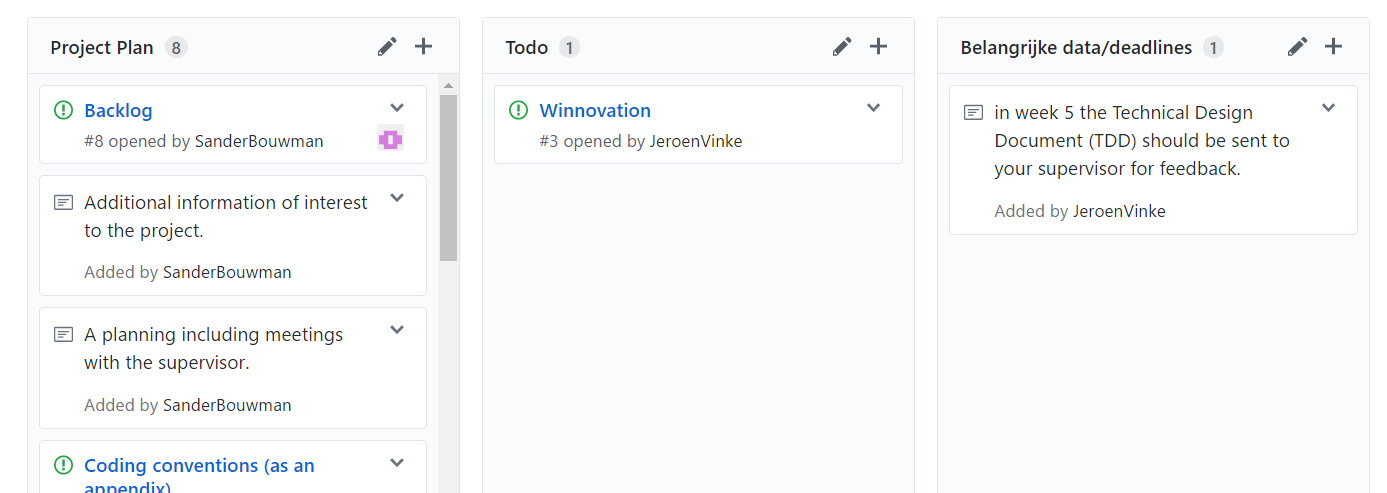
\includegraphics[angle=-90,origin=c,scale=0.75]
    {images/github-projects.PNG}
    \caption{GitHub project}\label{fig:githubproject}
\end{figure}

\end{document}